%%CHAP. Analysis

\begin{figure}[!ht]
        \subfigure{
        \centering
            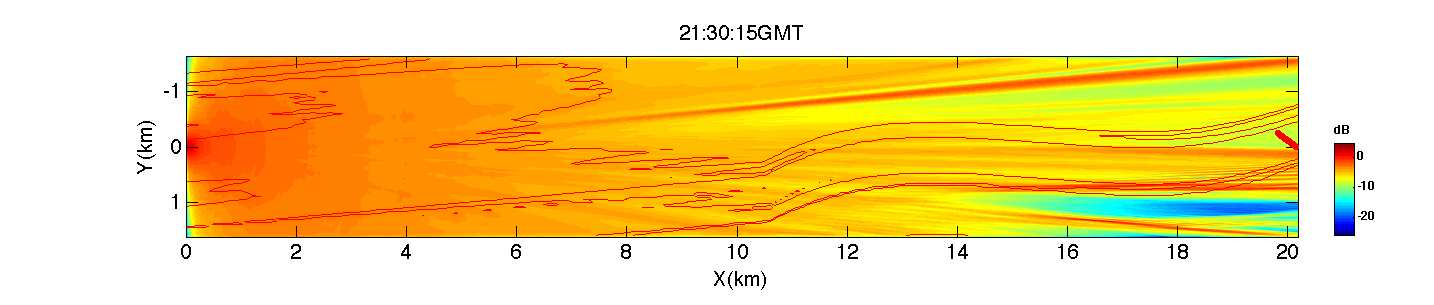
\includegraphics[width=0.8\textwidth]{sw06_event50_PE_NRL300_17Aug06_213015_curved.png}
            \label{fig:bf_pe_2130}}
        \subfigure{
            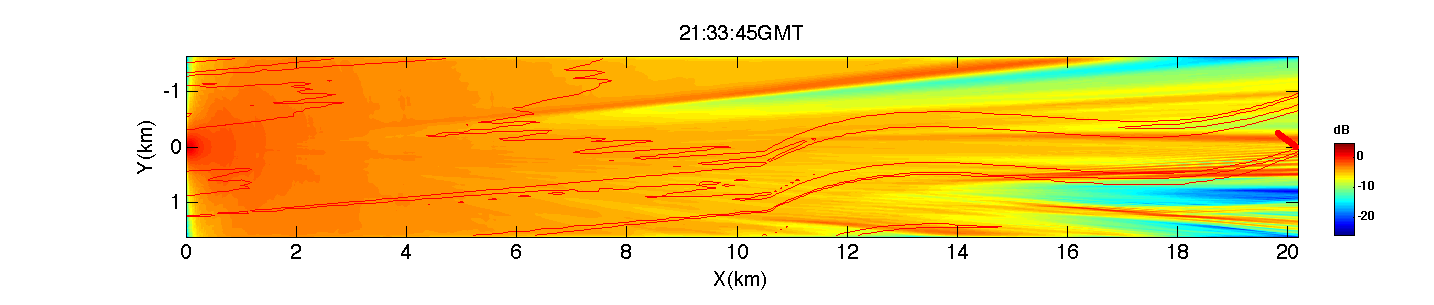
\includegraphics[width=0.8\textwidth]{sw06_event50_PE_NRL300_17Aug06_213345_curved.png}
            \label{fig:bf_pe_2133}}
    \caption{Depth integrated intensity from PE modeling results at 21:30:15GMT and 21:33:45GMT repectively, with a short white line indicating the length and direction of the Shark HLA}
    \label{fig:BE_pe_f3}
\end{figure}


\begin{figure}[!ht]
        \subfigure{
        \centering
            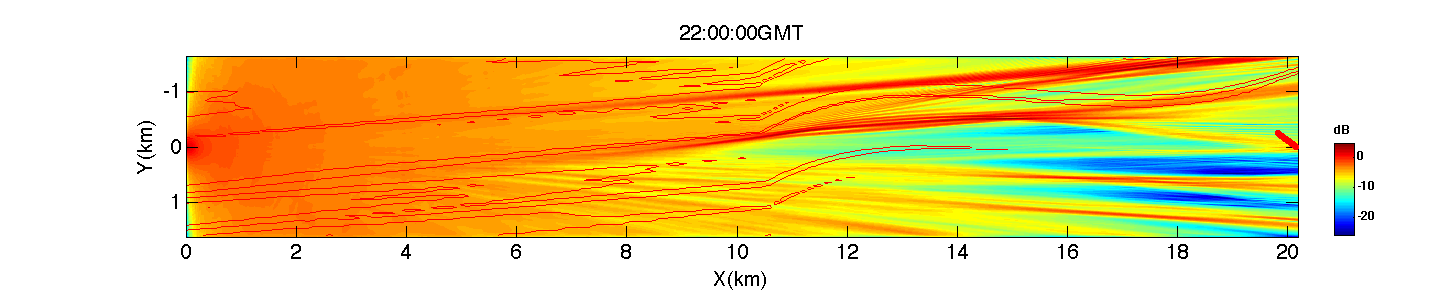
\includegraphics[width=0.8\textwidth]{sw06_event50_PE_NRL300_17Aug06_220000_curved.png}
            \label{fig:bf_pe_2200}}
        \subfigure{
            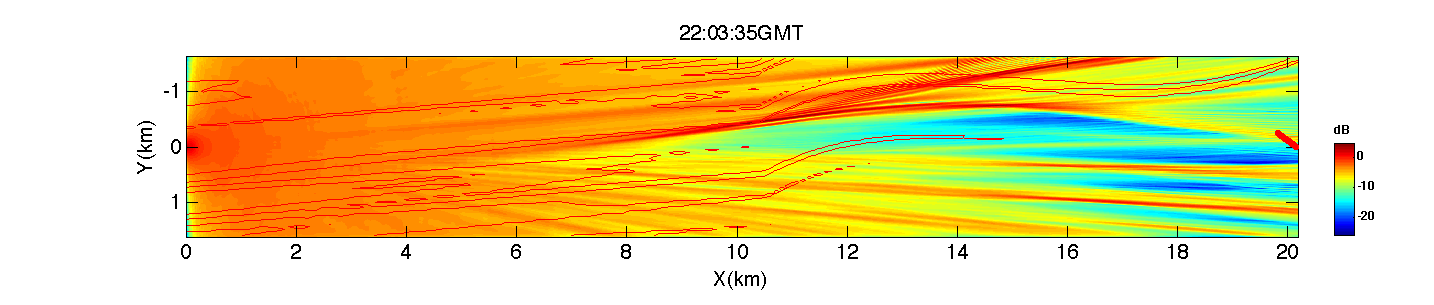
\includegraphics[width=0.8\textwidth]{sw06_event50_PE_NRL300_17Aug06_220335_curved.png}
            \label{fig:bf_pe_2003}}
    \caption{Depth integrated intensity from PE modeling results at 22:00:00GMT and 22:03:35GMT repectively, with a short white line indicating the length and direction of the Shark HLA}
    \label{fig:BE_pe_f4}
\end{figure}


\begin{figure}[!ht]
\begin{center}$
\begin{array}{rl}
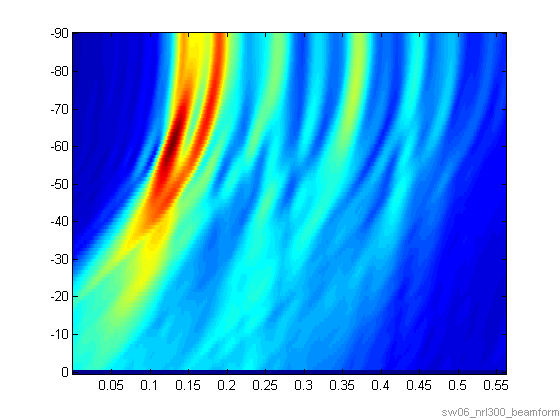
\includegraphics[width=0.5\textwidth]{sw06_nrl300_beamform_F3_ping019.png}&
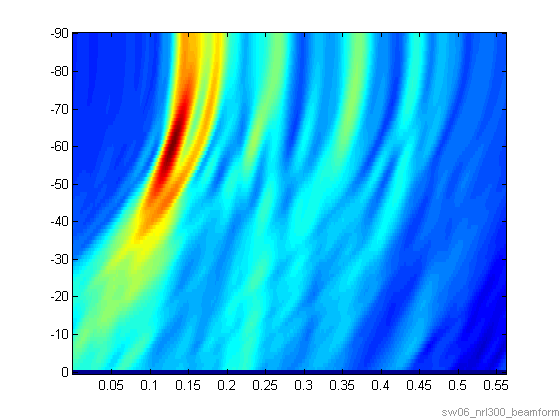
\includegraphics[width=0.5\textwidth]{sw06_nrl300_beamform_F3_ping031.png}\\
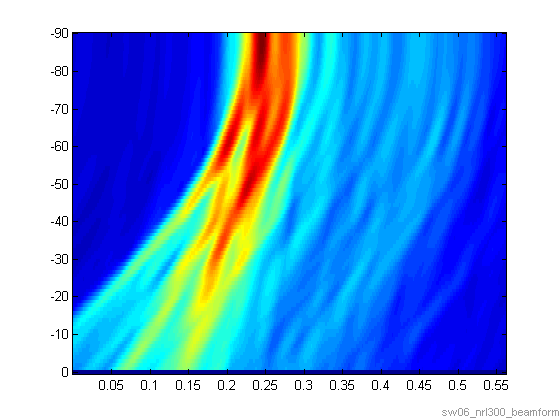
\includegraphics[width=0.5\textwidth]{sw06_nrl300_beamform_F4_ping010.png}&
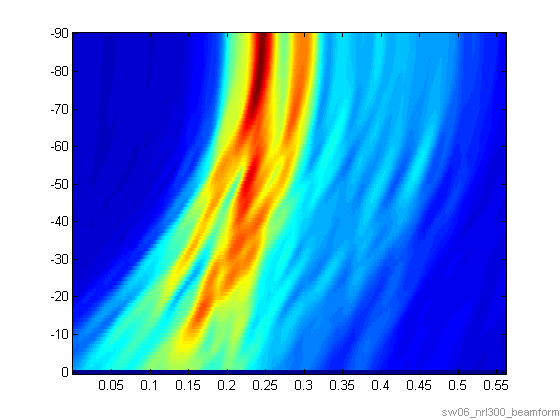
\includegraphics[width=0.5\textwidth]{sw06_nrl300_beamform_F4_ping041.png}
\end{array}$       
    \end{center}        
    \caption{Beamforming results on Shark HLA}
    \label{fig:BE_data}
\end{figure}

\begin{figure}[H]
  \centering
  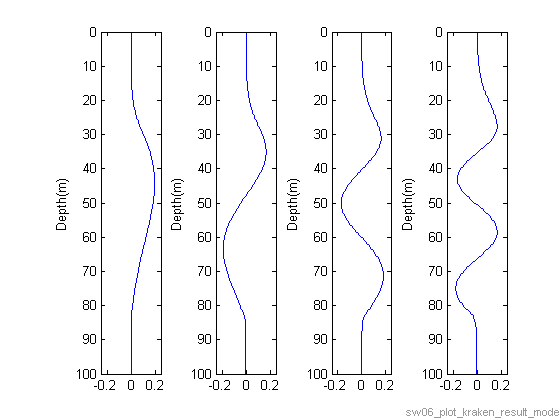
\includegraphics[width=0.8\textwidth]{kraken_results.png}
  \caption{From left to right, vertical modes 1-4 excited by a 330Hz frequency signal. Temperature data were recorded at NRL300 source, GMT21:30, Aug 17, 2006.}\label{fig:a2130}
\end{figure}


\begin{figure}[H]
  \centering
  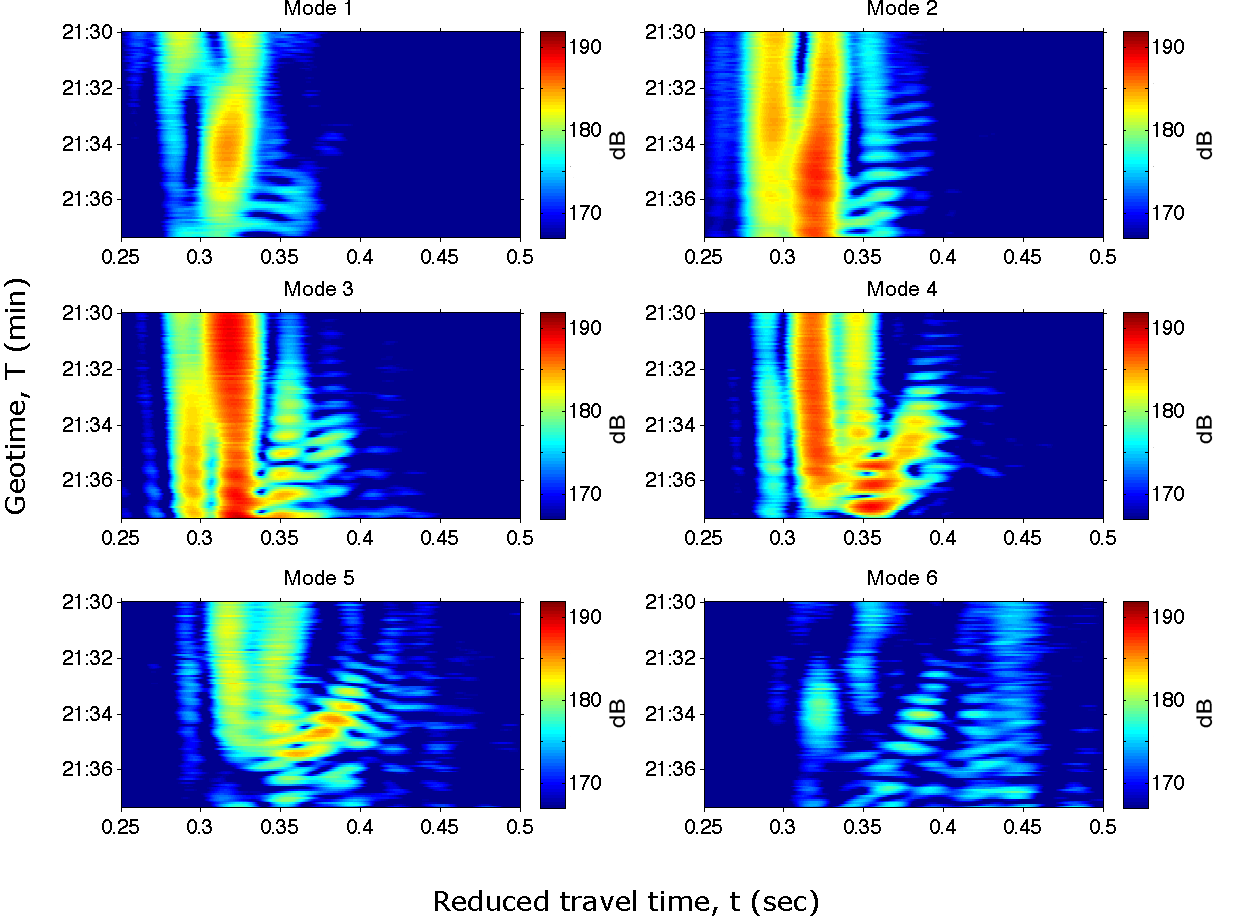
\includegraphics[width=\textwidth]{mode_6in1_ll_paper_small.png}
  \caption{Broadband model decomposition of acoustic signal from 21:30GMT to 21:37GMT (mode1-6).}\label{fig:a2130}
\end{figure}

\begin{figure}[H]
  \centering
  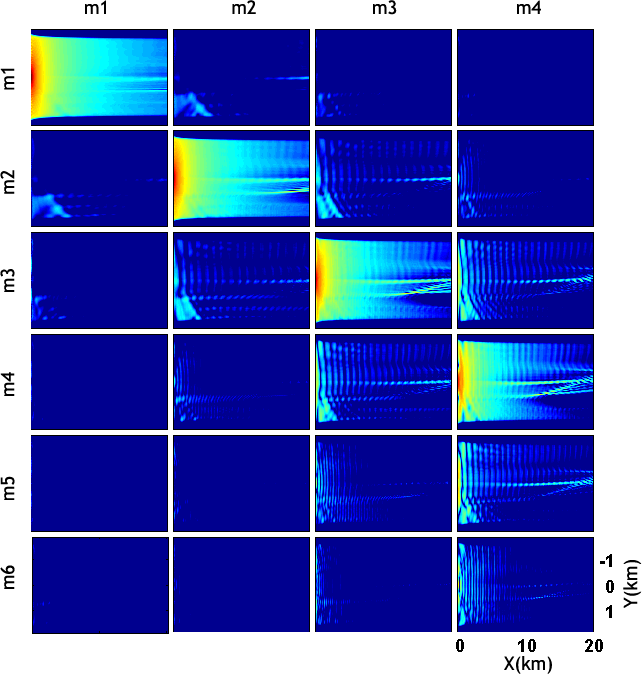
\includegraphics[width=\textwidth]{MC_213000_m_all_copy.png}
  \caption{PE modal coupling. From left to right, the excited modes at source; from top to bottom, the coupled modes. Most energy is confined at the excited mode at the source, which is consistent with the theory about adiabatic propagation at near-parallel environment.  Higher modes show stronger coupling effects than lower modes. Energy from mode 1 will couple to mode 3, while mode 4 can couple up to mode 8. }\label{fig:a2130}
\end{figure}


\begin{figure}[H]
  \centering
  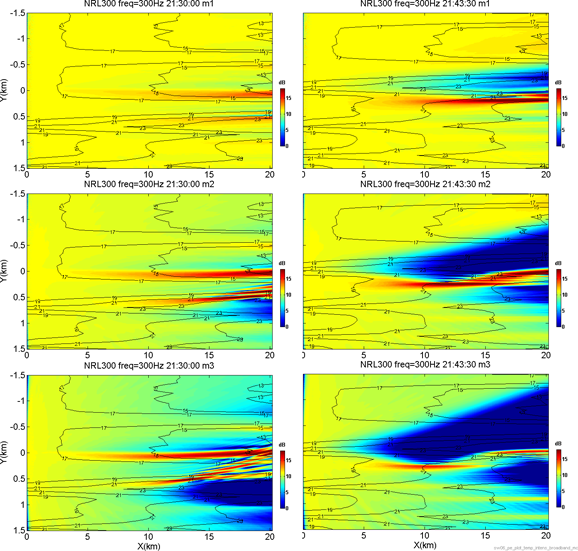
\includegraphics[width=\textwidth]{sw06_event50_PE_NRL300_300Hz_17Aug06_213000_MC_m1_3_copy_small.png}
  \caption{(Modal dependence) Acoustic intensity is shown for vertical modes 1~3 at GMT21:30:00(left) and GMT 21:43:40(right) respectively.  A single frequency signal (330Hz) source is placed at (0,0), depth = 70m. Temperature contour overlay shows the passing internal waves. }\label{fig:a2130}
\end{figure}


\begin{figure}[H]
  \centering
  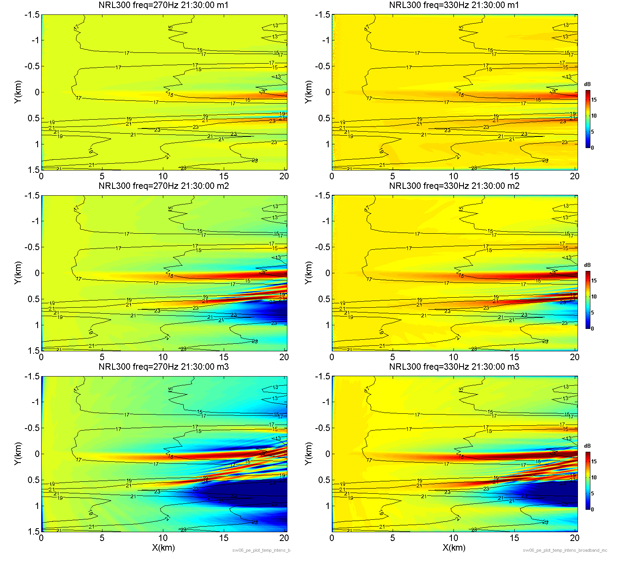
\includegraphics[width=\textwidth]{270_330_M1_3_213000_small.png}
  \caption{(Frequency dependence) Acoustic integrated sound intensity of vertical modes 1-3 at frequency = 270Hz, 330Hz at GMT21:30:00. Source position (x,y) = (0, 0) and source depth = 70m. Temperature contour overlay shows the passing internal waves. }\label{fig:a2130}
\end{figure}



\begin{figure}[H]
  \centering
  \includegraphics[width=\textwidth]{moving_pe.jpg}
  \caption{3-D PE modeling results showing the acoustic intensity and the temperature contour at depth 20 m.  Source is located at point (0,0) and white dashed lines indicate the acoustic track. }\label{fig:a2130}
\end{figure}

\begin{figure}[H]
  \centering
  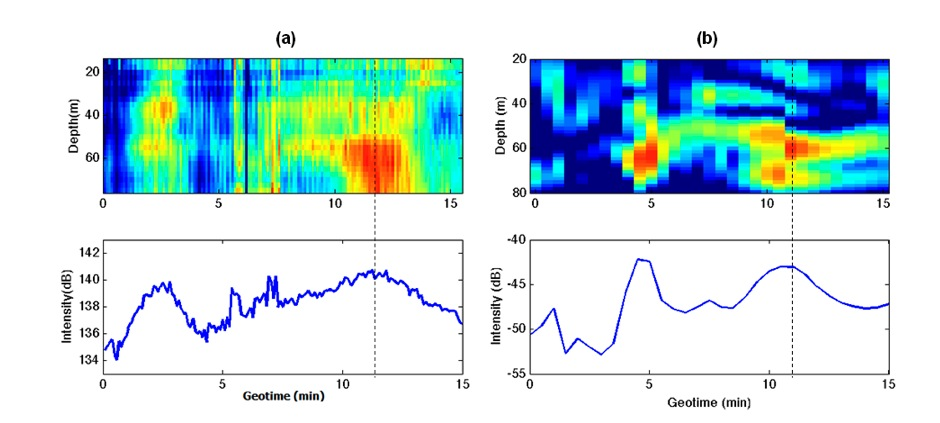
\includegraphics[width=\textwidth]{M3_comparison.jpg}
  \caption{(a) Data and (b) model comparison of the intensity as a function of depth (top panels) and depth-integrated intensity (bottom panels) on Zone 3, August 17, 2006 at 22:11 to 22:26 GMT.  The occurrence of focusing at geotime about 22:21:30 observed in the data was well predicted by the model.}\label{fig:a2130}
\end{figure}


\begin{figure}[H]
  \centering
  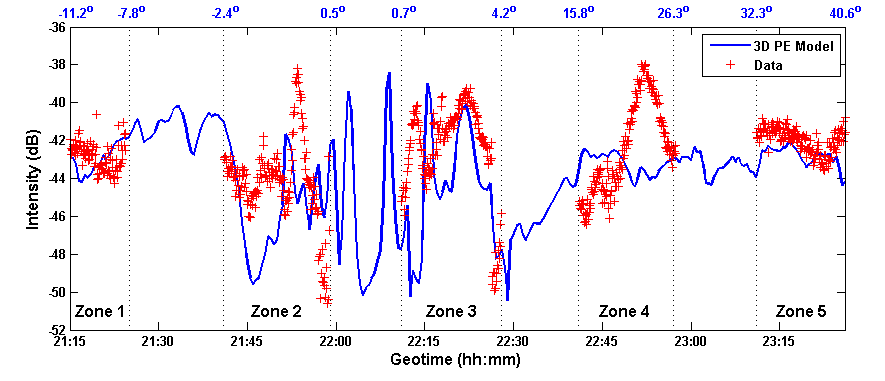
\includegraphics[width=\textwidth]{sw06_udel_pe_exp_comparison.png}
  \caption{PE model results and experiment data comparison for moving source J15. Solid line shows the results of 3D PE model. The propagating angles are shown at the top for the beginning and end of each transmission session}\label{fig:a2130}
\end{figure}

\begin{figure}[H]
	\centering
	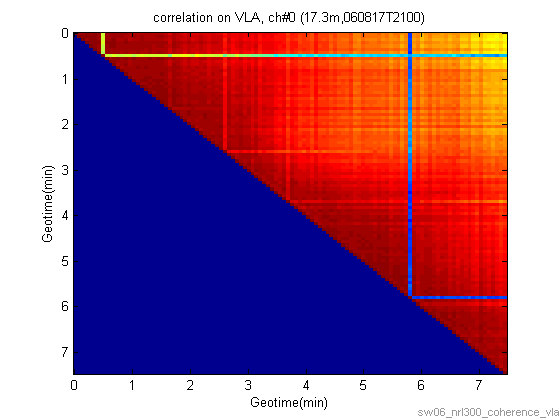
\includegraphics[width=0.5\textwidth]{060817T2100_ch00_vla_time_correlation.png}
	\caption{autocovariance function of channel 0 at 21:00}
\end{figure}

\begin{figure}[H]
	\centering
	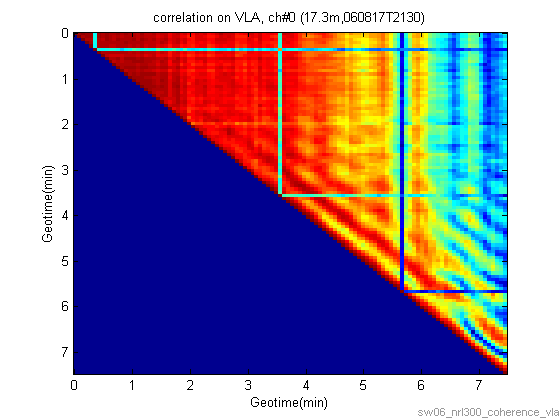
\includegraphics[width=0.5\textwidth]{060817T2130_ch00_vla_time_correlation.png}
	\caption{autocovariance function of channel 0 at 21:30}
\end{figure}

\begin{figure}[H]
	\centering
	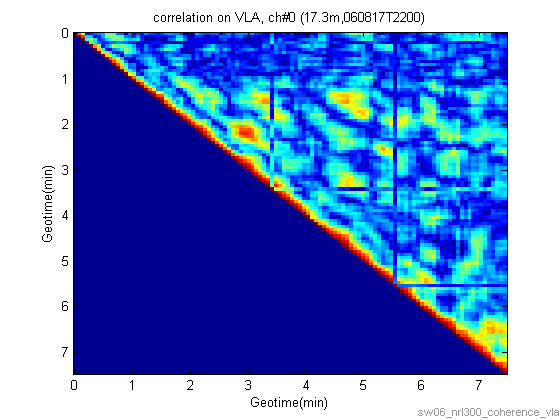
\includegraphics[width=0.5\textwidth]{060817T2200_ch00_vla_time_correlation.png}
	\caption{autocovariance function of channel 0 at 22:00}
\end{figure}